\chapter{The flags}
\label{chap:flags}

So, now that I have a reverse shell; how do I get the user and root flag? Luckily this first is rather easy. The reverse shell already gives me access to an user, \verb|www-data|. All that was left for this flag was to traverse to the \verb|/user/harim| folder, which would hold the \verb|user.txt| flag.

\vspace{5mm}

One flag down, one flag to go.

\section{Root}

The search for root started with the \verb|sudo -l| command. This listed that the current user (\verb|www-data|) had rights to use sudo without a password for \verb|/usr/bin/vi| and \verb|/var/www/html/*|. Vi being the famous text editor, and the html folder in which the Magento installation resides.

\begin{figure}[H]
	\centering
	\captionsetup{justification=centering}
	\noindent 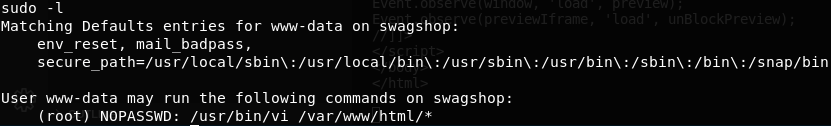
\includegraphics[width=\textwidth]{figures/sudo-output.png}
	\caption{\emph{The output of sudo -l.}}
	\label{fig:sudo}
\end{figure}

I figured this was no coincidence, and this would be the pivoting point to root. After some duckduckgo-ing around, I found an article on Medium\footnote{\url{https://link.medium.com/0dwd0VgL7Z}} about using Vim for privilege escalation. The user in the screenshots was \verb|haris|, which I suspect is actually this box.

The final example is about vim, and the output of \verb|sudo -l| actually looked really similar to mine. But this is where I went wrong, because the command \verb|sudo vi| didn't work. So I thought this was wrong, and started looking for other ways in.

\vspace{5mm}

In the end, I only had a few hours left before the box would be retired to find the root flag. I started to ask around on the Hack the Box forums, hoping to find some help to find the root flag. I got again nudged towards the sudoers file and Vim, which confused me. So, after a lot of playing around I found what I did wrong.

\begin{center}
    \verb|sudo vi| doesn't work. \verb|sudo /usr/bin/vi| does.
\end{center}

\begin{wrapfigure}{r}{4.5cm} % 4.5cm
	\centering
	\captionsetup{justification=centering}
	\noindent 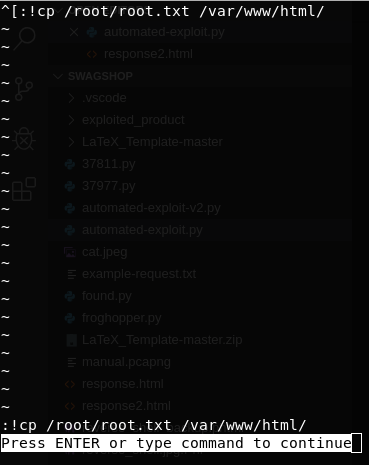
\includegraphics[width=\linewidth]{figures/root-copy-2.png}
	\caption{\emph{How I copied the file from within Vim.}}
	\label{fig:vimcopy}
\end{wrapfigure}

\vspace{2mm}

So, simple solution right? Just open the \verb|/root/root.txt| file with \verb|sudo /usr/bin/vi| and you have your flag. No. This actually was not allowed for some reason. So, what I ended up doing was copying the \verb|/root/root.txt| file to the \verb|/var/www/html| folder, and opening it there. This ended up giving me the root flag.

\begin{figure}[H]
	\centering
	\captionsetup{justification=centering}
	\noindent 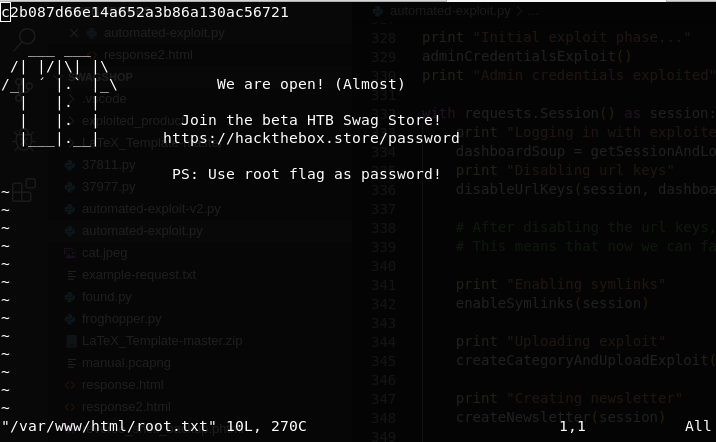
\includegraphics[width=\textwidth]{figures/root.png}
	\caption{\emph{The content of the root.txt file.}}
	\label{fig:root}
\end{figure}